%%%%%%%%%%%%%%%%%%%%%%%%%%%%%%%%%%%%%%%%%%%%%%%%%%%%%%
% A Beamer template for Ritsumeikan University       %
% Author: Ming-Hao Xu (Xu Minghao)                   %
% Date:   April 2022.                                %
% LPPL Licensed.                                     %
%%%%%%%%%%%%%%%%%%%%%%%%%%%%%%%%%%%%%%%%%%%%%%%%%%%%%%

\documentclass[10pt]{beamer}
\usepackage{hyperref}

\usepackage[UTF8]{ctex}
\usepackage[T1]{fontenc}

% other packages
\usepackage[superscript]{cite}
\usepackage{latexsym,amsmath,xcolor,multicol,booktabs,calligra}
\usepackage{graphicx,pstricks,listings,stackengine}
\usefonttheme[onlymath]{serif}

% dummy text; remove it when working on this template
\usepackage{lipsum}

\author{Wenchong Huang}
\title{Adaptive Mesh Refinement Design}
\institute{
    School of Mathematical Sciences, \\
    Zhejiang University.
}
\date{Mar. 8th, 2024}
\usepackage{Ritsumeikan}

% defs
\def\cmd#1{\texttt{\color{red}\footnotesize $\backslash$#1}}
\def\env#1{\texttt{\color{blue}\footnotesize #1}}
\definecolor{deepblue}{rgb}{0,0,0.5}
\definecolor{deepred}{rgb}{0.6,0,0}
\definecolor{deepgreen}{rgb}{0,0.5,0}
\definecolor{halfgray}{gray}{0.55}

\lstset{
    basicstyle=\ttfamily\tiny,
    keywordstyle=\bfseries\color{deepblue},
    emphstyle=\ttfamily\color{deepred},    % Custom highlighting style
    stringstyle=\color{deepgreen},
    numbers=left,
    numberstyle=\small\color{halfgray},
    rulesepcolor=\color{red!20!green!20!blue!20},
    frame=shadowbox,
}


\begin{document}

\begin{frame}
    \titlepage
\end{frame}

\begin{frame}[fragile]{研究背景}
    \footnotesize

    \begin{figure}[H]
        \centering
        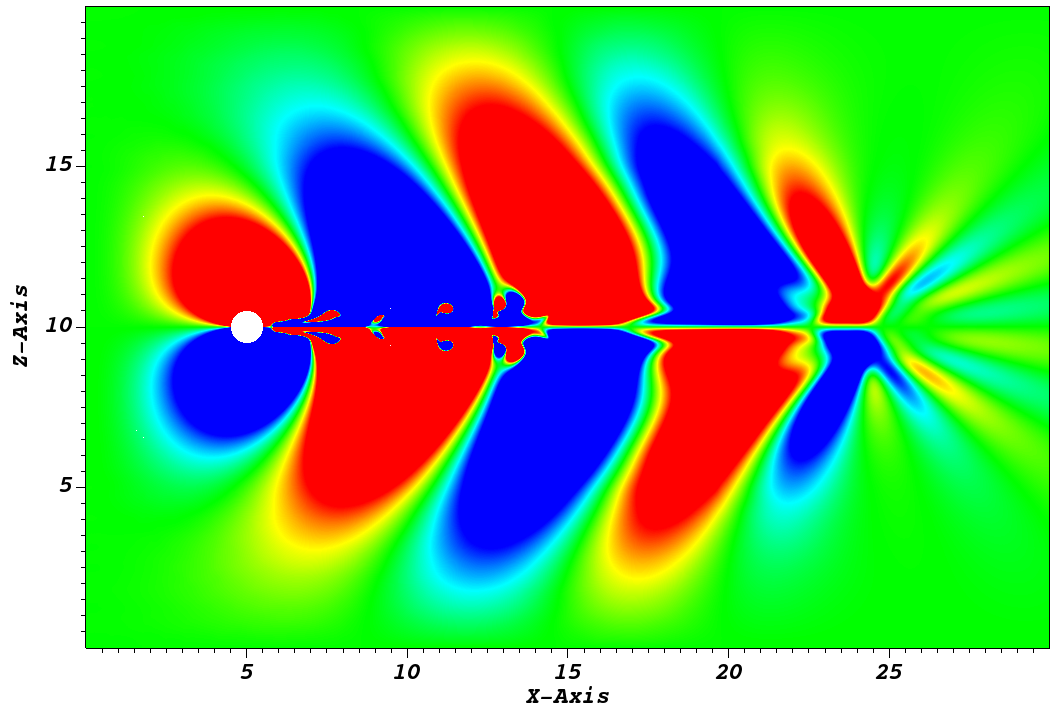
\includegraphics[width=0.3\textwidth]{png/densityPerturbation.png}
        \caption{\footnotesize 在密度分层流体中小球拖曳造成的密度扰动.}
    \end{figure}

    \vspace{-1em}

    \begin{figure}[H]
        \centering
        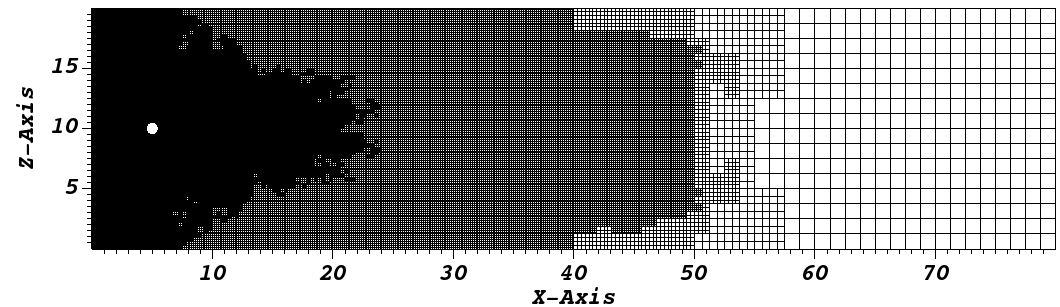
\includegraphics[width=0.8\textwidth]{png/amrdealii.png}
        \caption{\footnotesize Li 等人在捕捉小球拖曳尾涡时使用的网格.}
    \end{figure}

    \vspace{-1em}

    捕捉尾涡要非常细的网格,但全局用这么细的网格跑不动,加并行也没用。
    组里的代码目前不支持自适应,我们要解决这个问题。
\end{frame}

\begin{frame}[fragile]{AMR 简介}
    \footnotesize

    上世纪 90 年代, 美国 Lawrence Berkeley 国家实验室
    开发了一套支持基于块状加密的 AMR 网格与并行计算
    的基础软件设施库 Chombo\cite{ChomboDesign, ChomboAMR} . 

    \begin{figure}[H]
        \centering
        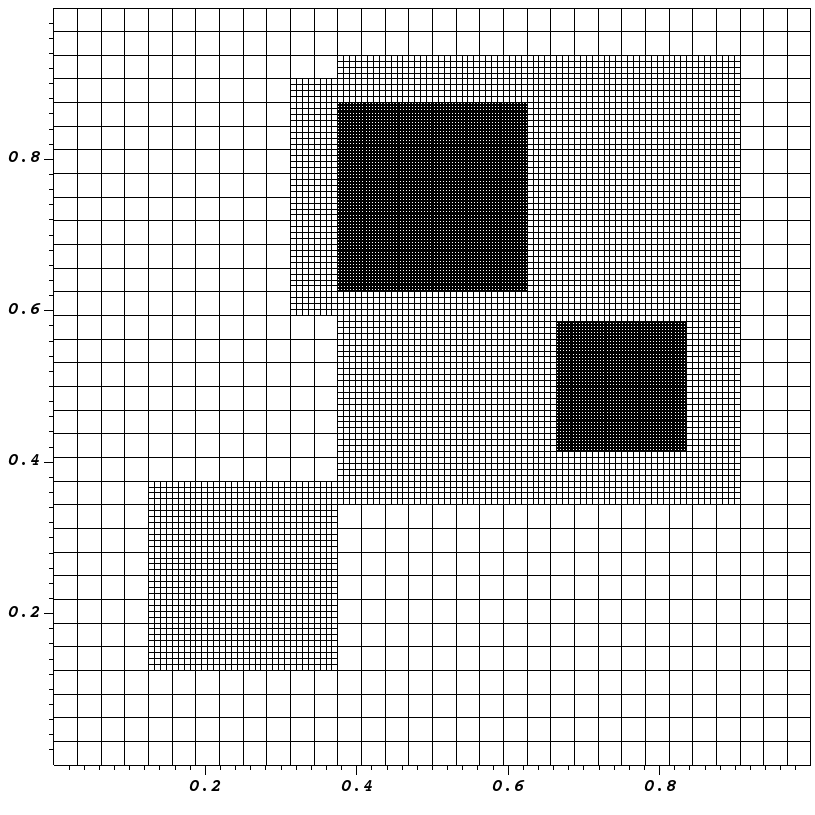
\includegraphics[width=0.4\textwidth]{png/blockAMR.png}
        \caption{\footnotesize 基于块状加密的 AMR 示意图.}
    \end{figure}

    用户可以选择物理区域中的若干个块状区域进行加密,
    每一个加密块在内存中都是连续的.
    用户还可以自定义加密率.

    \pause
    但是, Chombo 的代码实现过于老旧, 
    不符合现代编程理念.
    另外, 它将不规则边界当成一段一段的线段 \cite{ChomboEmbeddedBoundary},
    这导致它在不规则区域中不能做到高阶精度.
\end{frame}

\begin{frame}[fragile]{AMR 底层设计 —— 存储加密区域的布局}
    \footnotesize
    \textbf{组内程序}:用一个 \verb|Box| 存储一个矩形区域.

    \vspace{1em}
    \textbf{我们的设想}:用一个 \verb|BoxLayout| 封装同一层级的
    的所有块状加密区域,每个区域是一个 \verb|Box|,
    再用 \verb|std::vector<BoxLayout>| 存储整个区域.

    \begin{figure}[H]
        \centering
        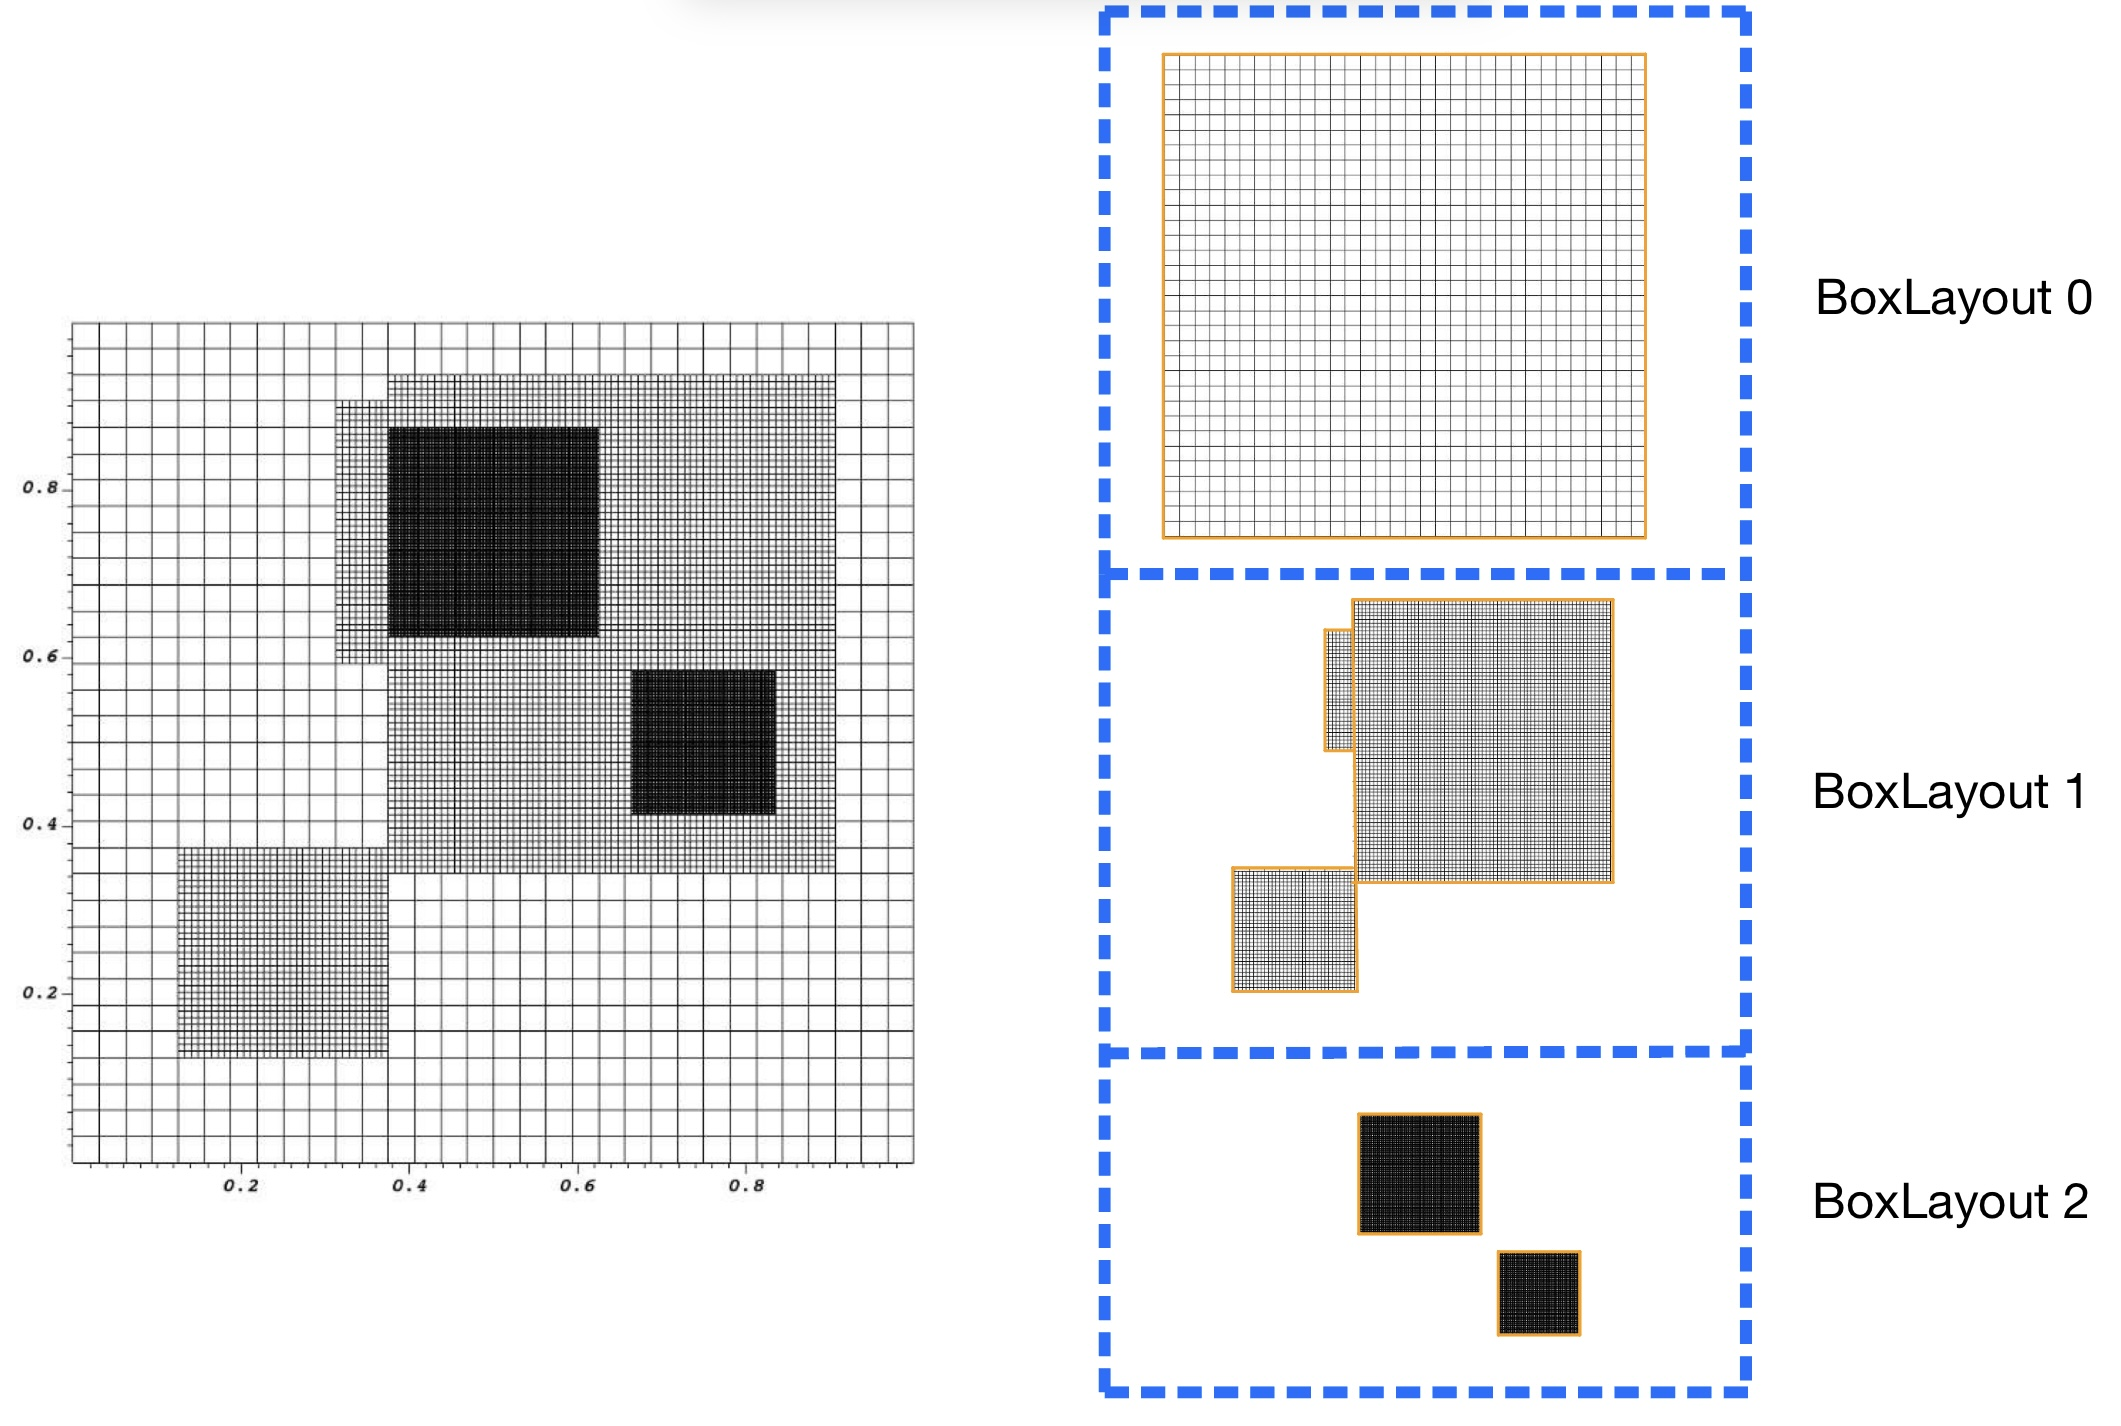
\includegraphics[width=0.7\textwidth]{jpg/BoxLayout.jpeg}
    \end{figure}

    \textbf{需要解决的问题}:\verb|BoxLayout| 内部用什么数据结构存储多个 \verb|Box| 更高效?
    当我要找一个网格时,需要快速知道它在哪个 \verb|Box| 里,
    如果每次找都要遍历一个层级里的所有 \verb|Box|, 当布局复杂时会很慢.
\end{frame}

\begin{frame}[fragile]{AMR 底层设计 —— 存储网格数据}
    \footnotesize
    \textbf{组内程序}:用一个 \verb|Tensor| 存储一个矩形区域中的所有数据.

    \vspace{1em}
    \textbf{我们的设想}:用一个 \verb|LevelData| 封装同一层级的
    的所有数据,\verb|LevelData| 内有多个 \verb|Tensor|,
    \verb|Tensor| 与 \verb|Box| 一一对应。
    再用 \verb|AllLevelData| 存储全部的数据.

    \vspace{1em}
    \verb|LevelData| 内部用数组存储多个 \verb|Tensor|,
    当要找某个网格数据时,先通过 \verb|BoxLayout| 的成员方法定位到 \verb|Box| 编号
    然后在对应的 \verb|Tensor| 里找就行。
\end{frame}

\begin{frame}[fragile]{AMR 底层设计 —— 存储算子}
    \footnotesize
    \textbf{组内程序}:用一个 \verb|SpatialOperator| 的派生类存储算子, 
    计算时先全部按标准格式计算, 然后左乘一个稀疏矩阵来校正不规则格点.
    稀疏矩阵在算子的构造函数中预处理.

    \vspace{1em}
    \textbf{不能直接推广的原因}:\verb|LevelData| 并不是 \verb|Tensor|,
    无法左乘稀疏矩阵, 而且算子的离散格式会用到不同层级的数据.

    \vspace{1em}
    \textbf{我们的设想}:设计一个 \verb|FillGhost| 类,它将每个 \verb|Box| 向外延拓两格,
    并且填充 Ghost Cell. 然后算子全部用标准格式计算. \verb|SpatialOperator| 及其派生类
    在架构层面不需要改太多.
\end{frame}

\begin{frame}[fragile]{AMR 中的高阶虚拟单元填充方法}
    \footnotesize
    要将 AMR 推广到高阶精度, 首先需要解决粗细网格交界处的虚拟单元填充问题.
    我们参考 Zhang 的工作\cite{Zhang2011} .
    以下图所示简单的二维情形为例, 白色是粗网格区域,
    灰色是细网格区域, 对于黑色三角形所示的细网格虚拟单元,
    我们可以用圆点所示的粗网格积分平均来拟合一个四阶多项式
    (当圆点落在灰色区域内部时, 指的是对应四个细网格积分平均的平均值),
    从而计算细网格虚拟单元的取值.
    
    \begin{figure}[H]
        \centering
        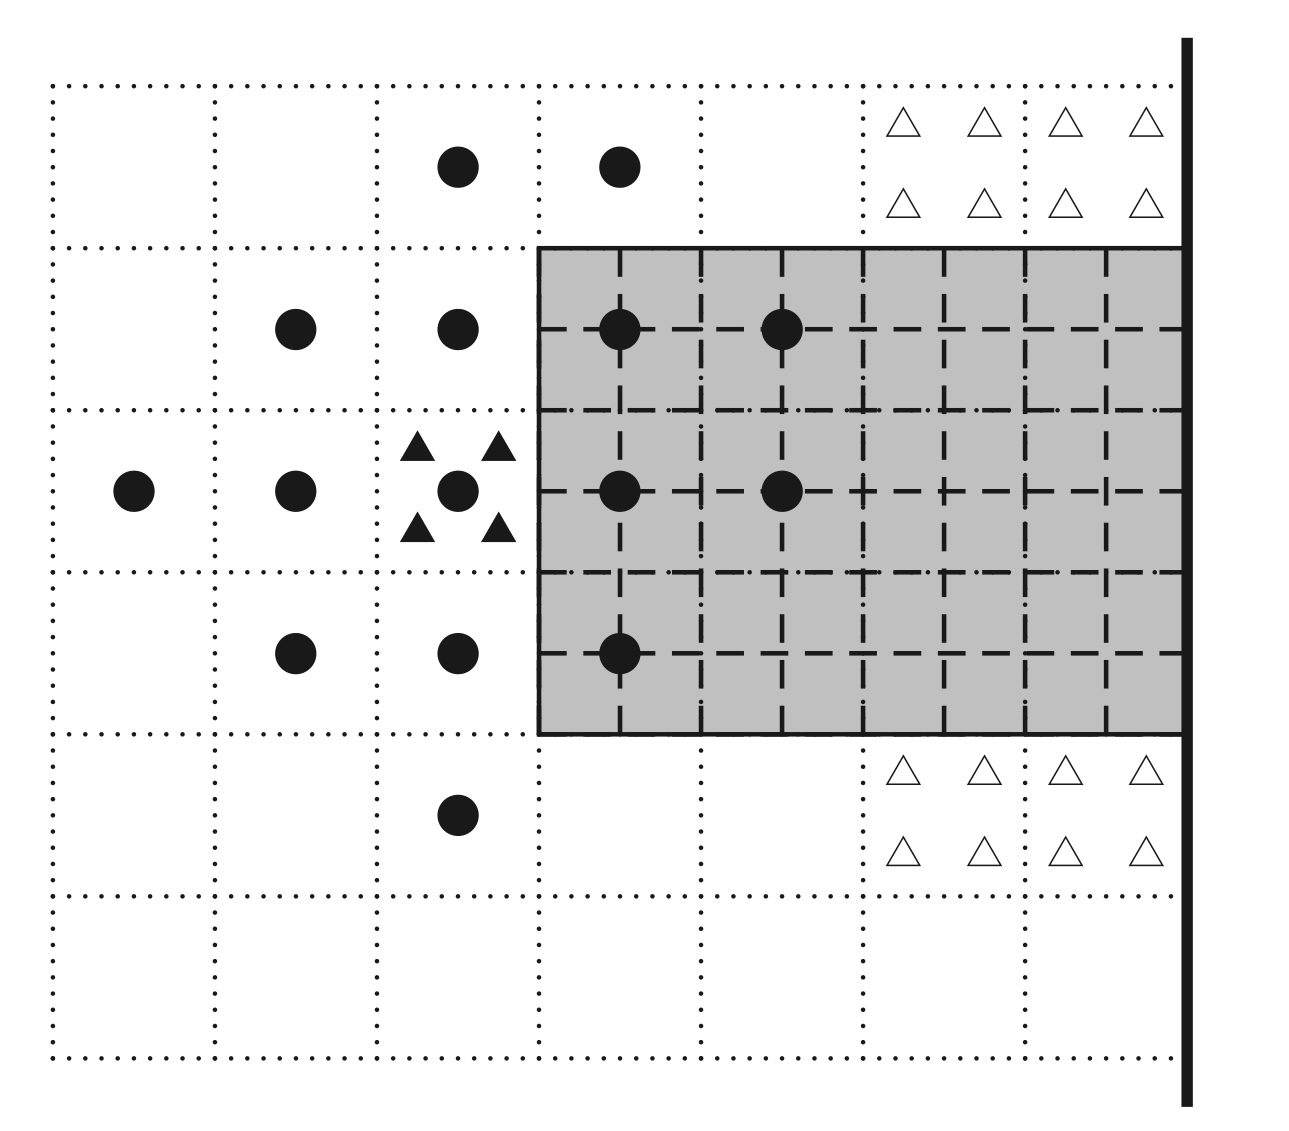
\includegraphics[width=0.4\textwidth]{jpg/fillGhost.jpeg}
        \caption{粗细网格交界处虚拟单元的填充示意图\cite{Zhang2011}}
    \end{figure}
\end{frame}

\begin{frame}[fragile]{不规则边界的处理}
    \footnotesize

    在非规则边界附近填充虚拟单元时, 
    需要拟合一个高阶多项式. 具体而言,我们知道一些点 
    $\mathbf{x}_1,...,\mathbf{x}_n$, 
    以及这些点处的函数值 $y_1,...,y_n$. 
    我们需要确定一个二元多项式 $p\in \mathbb{P}_k[x,y]$, 使得
    \begin{equation}
        \sum_{i=1}^n |p(\mathbf{x}_i)-y_i|^2
    \end{equation}
    取得最小值. 这是一个加权最小二乘问题, 
    与一维情形很不一样, 要想使得该问题有唯一解, 
    并不能随意取 $\binom{k+2}{2}$ 个点, 
    而应该按照某种规则来选择点. 
    另外, 这些点必须选在网格点上, 
    在不规则边界附近亦是如此, 
    这使得这个问题更加复杂.
    适定格点生成算法 (Poised Lattice Generation, PLG)\cite{PLG} 解决的
    就是如何选择这些点的问题.

    我们需要设计一种基于殷集表示\cite{YinSet2D} 与 PLG 算法
    的不规则边界处理方法.
    文章\cite{lzx}已经做了相关工作,
    我们需要让它能够支持并行计算与自适应网格.
\end{frame}

\begin{frame}[fragile]{预期目标与进度安排}
    \footnotesize

    中期检查之前, 完成自适应网格底层的设计, 
    实现虚拟单元的填充, 使程序能够根据任一场函数 $\mathbf{u}$ 
    在网格单元的积分平均来计算出 
    $\frac{\partial u_i}{\partial x_i}$、
    $\nabla\cdot \mathbf{u}$、$\Delta \mathbf{u}$ 
    在网格单元的积分平均. 

    \pause\vspace{1em}
    毕设结题之前完成 Dirichlet 边界条件、
    Neumann 边界条件下椭圆方程的四阶有限体积并行自适应求解器,
    能够支持任意复杂的不规则区域.
    进行充分的数值实验, 并验证四阶收敛性.

    \pause\vspace{1em}
    未来一年内完成无穿透、无滑移边界条件下, 
    二维不可压 Navier-Stokes 方程的四阶有限体积投影方法求解器, 
    能够支持任意复杂的物理区域, 能够支持自适应网格与 CPU 并行计算. 
    实现代码并测试卡门涡街等具有代表性的算例, 
    对时空一致四阶收敛性进行数值验证. 
\end{frame}

\begin{frame}[allowframebreaks]
    \tiny
    \bibliography{ref}
    \bibliographystyle{ieeetr}
    \nocite{*} % used here because no citation happens in slides
    % if there are too many try use:
    % \tiny\bibliographystyle{alpha}
\end{frame}


\begin{frame}
    \begin{center}
        {\Huge\calligra Thank You}
    \end{center}
\end{frame}

\end{document}
